\flushleft
\begin{minipage}{.57\textwidth}
\begin{Exercise}[label = wdsstrecke, title = Widerstandsstrecke, difficulty = 3, origin = IPhO 1996 ]
Bestimme den Widerstand zwischen den Punkten $A$ und $B$
	\end{Exercise}
\end{minipage}
\hfill
\begin{minipage}{.2\textwidth}
	\flushleft
	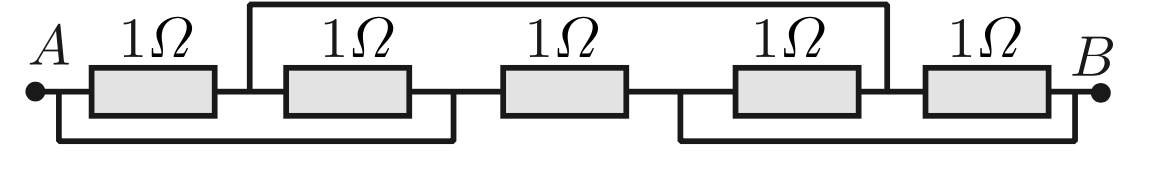
\includegraphics[scale = .2]{../tasks/ipho/wdsstrecke.png}
\end{minipage}
\begin{Answer}[ref = wdsstrecke]
	Um die Aufgabe einfach lösen zu können, muss man wissen, dass wen zwei Punkte nur durch einen Draht verbunden sind, sie auf dem gleichen Potential liegen müssen. Das liegt einfach daran, dass über ihnen keine Spannung abfallen kann, weil nichts da ist, an dem Spannung abfallen könnte \footnote{Außer natürlich der Draht selber. Aber in fast allen Aufgaben geht man davon aus, dass Drähte widerstandsfrei sind. Wenn das nicht so ist, sollte es auch angegeben sein.}\\
	Wir nennen diese Punkte $A$, $B$ und $C$ (siehe Abb.\ref{fig:wdsstreckeep}). Jetzt kann man einfach einen Stromkreis zeichnen, in dem es nur noch die Punkte $A$, $B$ und $C$ gibt. Dafür ist es hilfreich, wenn man die Widerstände nummeriert, sodass man sich nicht vertut. Wenn wir uns \ref{fig:wdsstreckeep} anschauen, dann stellen wir zuerst fest, dass $A$ mit $C$ durch die Widerstände 1 und 2 verbunden ist, $A$ mit $B$ durch 3 und $B$ mit $C$ durch die Widerstände $4$ und $5$. \\
	Der neue Stromkreis sieht dann so aus, wie in Abb.\ref{fig:wdsstreckes} gezeigt. Hier können wir jetzt mit den ganz normalen Regeln für Reihen- und Parallelschaltungen arbeiten. Die Widerstände 4 und 5 sind parallel geschaltet, die Widerstände 1 und 2 auch, und die Ersatzwiderstände für diese beiden Parallelschaltungen sind gemeinsam in Reihe parallel zu dem Widerstand 3 geschaltet.
	Damit ist der Gesamtwiderstand
	\begin{equation*}
		\boxed{
			\frac{1}{R_{AB}} =\underbrace{\frac{1}{R}}_{Wds. 3} + \overbrace{\frac{1}{\underbrace{\frac{R}{2}}_{1\parallel 2}+\underbrace{\frac{R}{2}}_{4\parallel 5}}}^{Wds.~parallel~zu~3} \Rightarrow R_{AB} = \frac{R}{2} = 0.5~\Omega,
			}
	\end{equation*}
	wobei mit einem Einzelwiderstand von $ R = 1~\Omega$ gerechnet wurde, wie in der Skizze zur Aufgabenstellung gezeigt.
\end{Answer}
\begin{figure}[h]
	\begin{subfigure}[b]{0.5\textwidth}
		\centering
		  \ctikzset{bipoles/resistor/width=0.4}
\begin{tikzpicture}
	\draw
		\foreach \h in {1,2,3,4,5}
		{(\h-1,0) to[/tikz/circuitikz/bipoles/length=25pt, R] (\h,0)};
	\foreach \h in {0,1,2,3,4,5}
	{\filldraw[black] (\h,0) circle (1.5pt);}
	\node at (-0.2,0) {$A$};
	\node at (5.2,0) {$B$};
	\node at (1,0.3){$C$};
	\node at (2,-0.3){$A$};

	\node at (3,-0.3) {$B$};
	\node at (4,0.3) {$C$};
	\draw (0,0) -- (0,0.5) -- (2,.5)--(2,0);
	\draw (1,0) -- (1,-.5) -- (4,-.5) -- (4,0);
	\draw (3,0) -- (3,.5) -- (5,.5)--(5,0);
	\foreach \h in {1,2,3,4,5}
	{\node at (-0.5+ \h,0) {\footnotesize \h};}

	
	 
	

\end{tikzpicture}
		\caption{Punkte auf gleichem Potential}
		\label{fig:wdsstreckeep}
	\end{subfigure}
	\begin{subfigure}[b]{0.5\textwidth}
		\centering
		  \ctikzset{bipoles/resistor/width=0.4}
\begin{tikzpicture}
	\draw
	(0,0) to[/tikz/circuitikz/bipoles/length=25pt, R] (1,0)
	(0,-0.5) to[/tikz/circuitikz/bipoles/length=25pt, R] (1,-0.5)
	(1,0) to (1.5,0)
	(0,0) to (0,-0.5)
	(1,-.5) to (1,0)
	(0,-.5) to (0,-1)
	(0,-1) to[/tikz/circuitikz/bipoles/length=25pt, R] (1.5,-1)
	(1.5,-1)to[/tikz/circuitikz/bipoles/length=25pt, R](1.5,0)
	(1.5,0) to (2,0)
	(1.5,-1) to (2,-1)
	(2,0) to[/tikz/circuitikz/bipoles/length=25pt, R] (2,-1)
	;
	\filldraw[black] (0,0) circle (1.5pt);
	\filldraw[black] (1,0) circle (1.5pt);
	\filldraw[black] (1.5,-1) circle (1.5pt);
	\node at (0,0.3) {$A$};
	\node at (1,0.3) {$C$};
	\node at (1.5,-1.3) {$B$};
	\node at (0.5,0) {\footnotesize 1};
	\node at (0.5,-.5) {\footnotesize 2};
	\node at (0.75,-1) {\footnotesize 3};
	\node at (1.5,-0.5) {\footnotesize 4};
	\node at (2,-0.5){\footnotesize 5};
	
\end{tikzpicture}
		\caption{vereinfachter Stromkreis}
		\label{fig:wdsstreckes}	
	\end{subfigure}
	\caption{Skizzen zum Aufbau}
\end{figure}
	
